\documentclass{article}
\usepackage[margin=.5in]{geometry}
\usepackage{graphicx, dblfloatfix}
\usepackage{amsmath, amssymb, amsfonts, mathrsfs, mathtools, physics}
\usepackage[english]{babel}
\usepackage[autostyle, english = american]{csquotes}
\usepackage[normalem]{ulem}
\usepackage[title,titletoc,toc]{appendix}
\usepackage{pgfplotstable}
\usepackage{array, booktabs, colortbl}
\MakeOuterQuote{"}

\pgfplotsset{compat=1.12}


\newcommand{\redchi}{$\tilde{\chi}^2\,$}
\DeclareMathOperator{\cov}{cov}
\DeclarePairedDelimiter{\parens}{\lparen}{\rparen}

\newcommand{\twohalff}[2]{$5^2 #1_{1/2},\, f = #2$}
\newcommand{\twohalf}[1]{$5^2 #1_{1/2},\, f = 2$}

\title{Optical Pumping}
\author{Aman LaChapelle}

\begin{document}
\raggedright
\maketitle

\begin{abstract}
  We will show that doppler broadening due to thermal fluctuations can be alleviated in order to show spectral features that would otherwise be hidden.  In this case, we will show measurement of the hyperfine states of Rubidium (whose linewidth requires higher resolution than the doppler broadening allows) in order to demonstrate this technique.
\end{abstract}

\tableofcontents
\newpage

\section{Introduction}
  We show that it is possible to spectally resolve features of the Hyperfine structure of Rubidium that would otherwise be impossible outside some sort of atomic trap using a technique called doppler-free spectroscopy.  We also show that it is possible to make use of the interference pattern of a Michelson Interferometer to make calibrations and create a conversion from time into frequency for the purposes of measurement on a time-resolved oscilloscope.  This means that we can use an oscilloscope with (potentially) much better-resolved time dynamics to mimic the purpose of a spectrum analyzer.

  \hspace{.25cm}

  In particular, we discuss the methods used for finding the information required, including the methods used to find the Hyperfine transitions, measure the linewidth of the resonances, and the linewidth of the doppler-broadened peak.

\section{Theory}
  \subsection{Energy of Rb}
  Rubidium is often used as an atom for optical experiments because it has a hydrogen-like spectrum in its ground state, which allows for the splitting and simplification of the system hamiltonian.  If we ignore the relativistic effects and assume that the nucleus is much heavier than the outer electrons, we can write the Hamiltonian of the system as the sum of different parts.  We have
  \begin{gather*}
    H_{kin} = \frac{p^2}{2m} \\
    H_{em} = \frac{-Z_{ef\!f}e^2}{4\pi\epsilon_0r} \\
    H_{so} = \frac{1}{m_e e c^2}\frac{1}{r}\pdv{V}{r}\vec{L} \\
    H_{hyp, 1} = \alpha \vec{J}\cdot\vec{I} \\
    H_{hyp, 2} = \frac{\beta}{2I(2I-1)j(2j-1)}\parens*{3(\vec{I}\cdot\vec{J})^2 + \frac{3}{2}(\vec{I}\cdot\vec{J}) - I(I+1)j(j+1)}
  \end{gather*}

  The first three are fairly basic - they stem from the electron's motion and interactions between the electron's magnetic moment and the magnetic moment of its motion around the nucleus.  They are the standard additions to the Hydrogen atom hamiltonian with the exception of the relativistic correction term.

  \hspace{.25cm}

  The second two are more complex.  $H_{hyp, 1}$ is the hyperfine interaction that occurs between the electon's total angular momentum $\vec{J} = \vec{L} + \vec{S}$ and the atom's intrinsic nuclear spin $\vec{I}$.  The constant $\alpha$ is called the magnetic hyperfine structure constant.  This interaction is also present in other atoms, but we see it very prominently in atoms like Rb due to the fact that the outer valence electrons typically have very high $\ell$ (hereafter the quantum number associated with $\vec{L}$) states, which directly increases j (quantum number associated with $\vec{J}$), it is a magnetic dipole interaction.  Along that same vein, we have $H_{hyp, 2}$.  It is the interaction between the electric quadrupole moment of the nucleus and the electron.  The dipole moment of the interaction is given in $H_{em}$.  As with any other separable hamiltonian, we can apply non-degenerate perturbation theory and calculate the energy shift due to the perturbation quite simply.  Thus we can simply write down the energy of the system as
  \begin{equation*}
    E_{tot} = E_0 + E_{hyp}
  \end{equation*}
  where we have wrapped all the non-hyperfine parts into one term, and the two hyperfine hamiltonians into the $E_{hyp}$ term.

  \hspace{.25cm}

  \subsection{Electron Transitions}
  The ground state for 85Rb and 87Rb is the \twohalf{S} state.  Recall spectroscopic notation: $n^{2s+1}\ell_{j}$.  Since we are measuring the hyperfine transitions between the \twohalf{P} states, we need some way to get the electrons into that state.  We do this with a pump beam.  In the orientation that we use, we happen to use the pump beam reflected and passed through a linear polarizer as our probe beam, but this is not neccesary.  We pump the ensemble into the \twohalf{P} states with a 780 nm laser.  From there we let the hyperfine splitting occur as it normally would.

  \hspace{.25cm}

  The pump beam pumps the atoms into a certain state, but the probe beam is what we measure.  What we actually measure is the intensity of the probe beam as it passes through the sample, and then invert that signal on our instrumentation in order to plot the atoms' absorbtion of photons as a function of time (and since the laser sweeps frequencies as a function of time, frequency as well).  In the particular case of the hyperfine transition peaks, for example, we see absorbtion dips \textbf{at} the transition energies, because the atoms have nowhere to go and thus the photons simply pass through.  We can then find the difference in frequency between hyperfine states by measuring the difference between the times at each peak tip and from that converting into frequency.  We measure the splitting between the \twohalff{P}{0} and the \twohalff{P}{3} in integer increments in this way.

  \subsection{Doppler Broadening}
  Since the atoms are moving back and forth quite quickly at room temperature inside the vapor cell, there must be a consideration of the doppler shift on photons from the laser as seen by the atoms as well as photons emitted from the atoms.  In both cases, if there is a component of velocity pointed parallel or antiparallel to the pump/probe beams, we will see a broadened spectrum that is essentially useless.  There are a few methods to take care of this issue.  The first is to stop the atoms.  This is usually accomplished with a MOT (Magneto-Optical Trap), which uses magnetic fields and radiation pressure with lasers to cool the atoms to lower kinetic energy states.  This is usually the path taken to study the physics of ultracold atoms, and to study properties such as the Bose-Einstein condensate.  Atoms can be further cooled in order to reduce their velocity even more with evaporative cooling which involves simply allowing the 'hot' atoms to simply escape the trap.

  \hspace{.25cm}

  Clearly we are not going to that much trouble in this particular experiment, we have a different objective.  We want to measure an effect with a linewidth of roughly 36 MHz which is not terrible compared to other effects in atomic physics (for example, Rydberg transition linewidths which are commonly in the kHz range).  Thus we use this technique of Doppler-Free Spectroscopy.  The idea is that if we pass the same laser through the atoms twice, first as a pump beam and then at reduced intensity as the probe beam, we will be able to see dips in absorbtion at the finer spectral features.  If the pump beam fully saturates the sample, then we will see less absorbtion of the probe beam at the energies where the hyperfine states live.  These states corresponds to the atoms that are not moving - there is a perpendicular doppler shift, so the atoms must truly not be moving almost at all.  If an atom is in resonance with a doppler-shifted beam, then it will not be in resonance with the beam that is reflected in the probe, so there will be no attenuation of absorbtion at that frequency.

  \hspace{.25cm}

  Thus we are able to pick out the individual hyperfine states by essentially picking the spectrum from only the atoms that don't move, removing the need for a MOT by simply choosing the ones that we want to look at.

  \hspace{.25cm}

  We can characterize the doppler broadening in terms of frequency, and write the full width at half max as
  \begin{equation}
    \Gamma = 2\frac{\nu_0}{c}\parens*{\frac{2k_BT}{M}\ln{2}}^{1/2}.
    \label{doppler}
  \end{equation}
  We can derive this relation from the Boltzmann distribution - given that the atoms are in some thermal state we can describe the probability distribution of their velocities with the Boltzmann distribution.  We will refrain from deriving this relation here, however.

  \subsection{Crossover Frequencies}
  Occasionally there are atoms whose transitions are in resonance with a doppler-shifted frequency, and there will be another transition that is in resonance with the frequency with the opposite doppler shift.  This will cause what are known as crossover frequencies, which occur exactly halfway between two hyperfine transitions.  This becomes important as we begin to examine the spectrum, but in essence as long as we realize that the outermost features are hyperfine features, and knowing that the crossovers happen at exactly halfway between hyperfine features we can pinpoint which are hyperfine and which are crossover features.

\section{Experimental Methods}
  \subsection{Apparatus}
  It will be much simpler to explain the components of the optical setup if there is something to refer to, so here we will show a rendering of the optical table as seen from above.

  \begin{figure}[!htb]
    \centering
    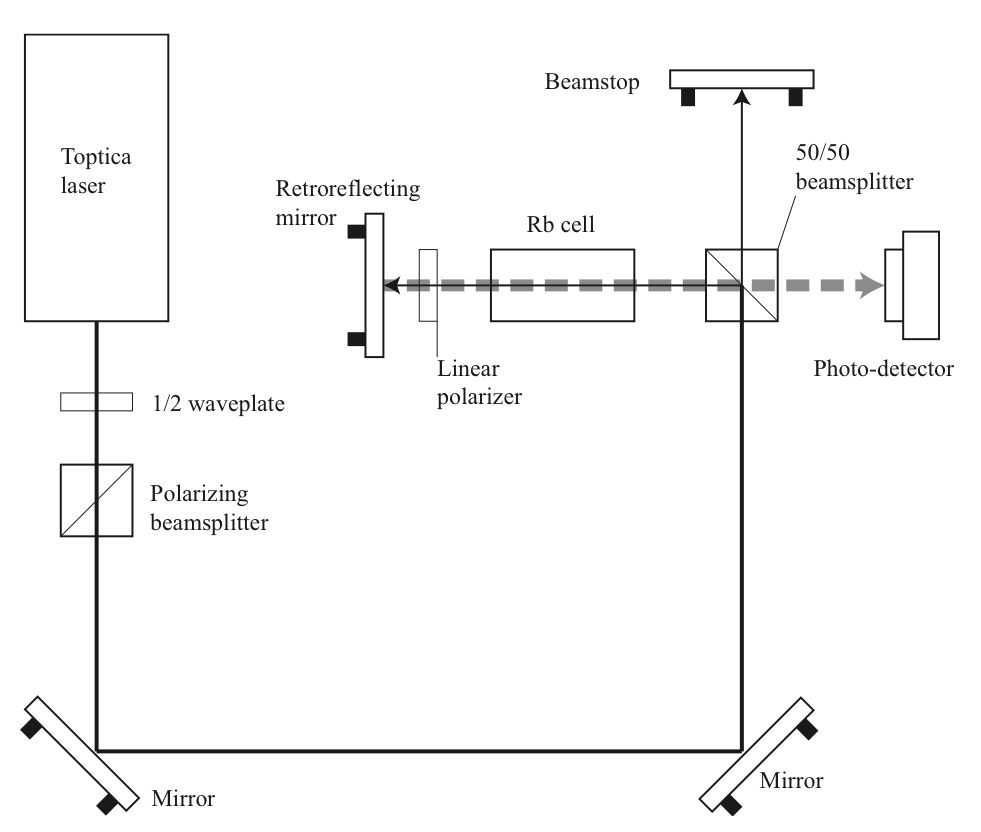
\includegraphics[scale=.25]{hyperfine_apparatus.png}
    \caption{A depiction of the optical table as seen from above.  The dark dashed arrow corresponds to the pump beam, while the lighter dashed arrow corresponds to the probe beam.}
    \label{apparatus}
  \end{figure}

  If we refer to Figure~\ref{apparatus}, we will notice that we use a Michelson Interferometer to perform both a calibration and the Doppler-Free Spectroscopy.  In performing the spectroscopy, we can simply trace the beam from its source.  All the components that lead the laser into the interferometer are simply to send the laser into this particular experiment as opposed to a setup that is across the table.

  \hspace{.25cm}

  As the laser enters the interferometer, we will notice that the beam is split in two directions.  In one direction, the beam simply reflects off a retroreflecting mirror and returns to the beam splitter to recombine with the other arm.  The vapor cell arm of the interferometer consists of the vapor cell itself, a linear polarizer and another retroreflecting mirror.  After the pump beam passes through the vapor cell, it passes through a linear polarizer to reduce the intensity of the reflected beam which we use to probe the system.  The probe beam and the reflected beam from the other arm of the interferometer recombine at the beam splitter and from there head into the detector.  The detector sends a voltage signal to the oscilloscope, which then displays the signal in a time-resolved way.

  \hspace{.25cm}

  The laser sweeps over a range of frequencies in a saw-tooth pattern, such that at some given time (modulo one period) the laser will be at a given frequency.  We can calibrate this with the Michelson interferometer.  We must realize that the scope trace - the absorbtion spectrum - is importantly time-resolved because the atoms are resonant at certain laser frequencies, which will correspond to different times in our calibration.

  \subsection{Michelson Interferometer Calibration}
  We can calibrate the time axis of the scope trace using the interference pattern given by the Michelson interferometer.  There is a simple formula to calculate the difference in frequency between the two interferometer arms having to do with the phase difference:
  \begin{equation*}
    \Delta \phi = \frac{4\pi f}{c}\parens*{L_1 - L_2}
  \end{equation*}
  which leads to the relation (given that the spacing between maxima on the interference pattern is a multiple of $2\pi$)
  \begin{equation}
    \Delta f = \frac{c}{2\parens*{L_1 - L_2}}
    \label{interference}
  \end{equation}
  Making use of Eq.~\ref{interference}, we can calculate a value for the frequency spacing between interference maxima given lengths for our particular interferometer.  We measured
  \begin{gather*}
    L_1 = 29.5 \pm 0.5 \, cm \\
    L_2 = 10.5 \pm 0.5 \, cm
  \end{gather*}
  which results in a frequency spacing between maxima of
  \begin{equation}
    790 \pm 40 \, M\!H\!z.
    \label{freq_conv}
  \end{equation}

  \begin{figure}[!htb]
    \centering
    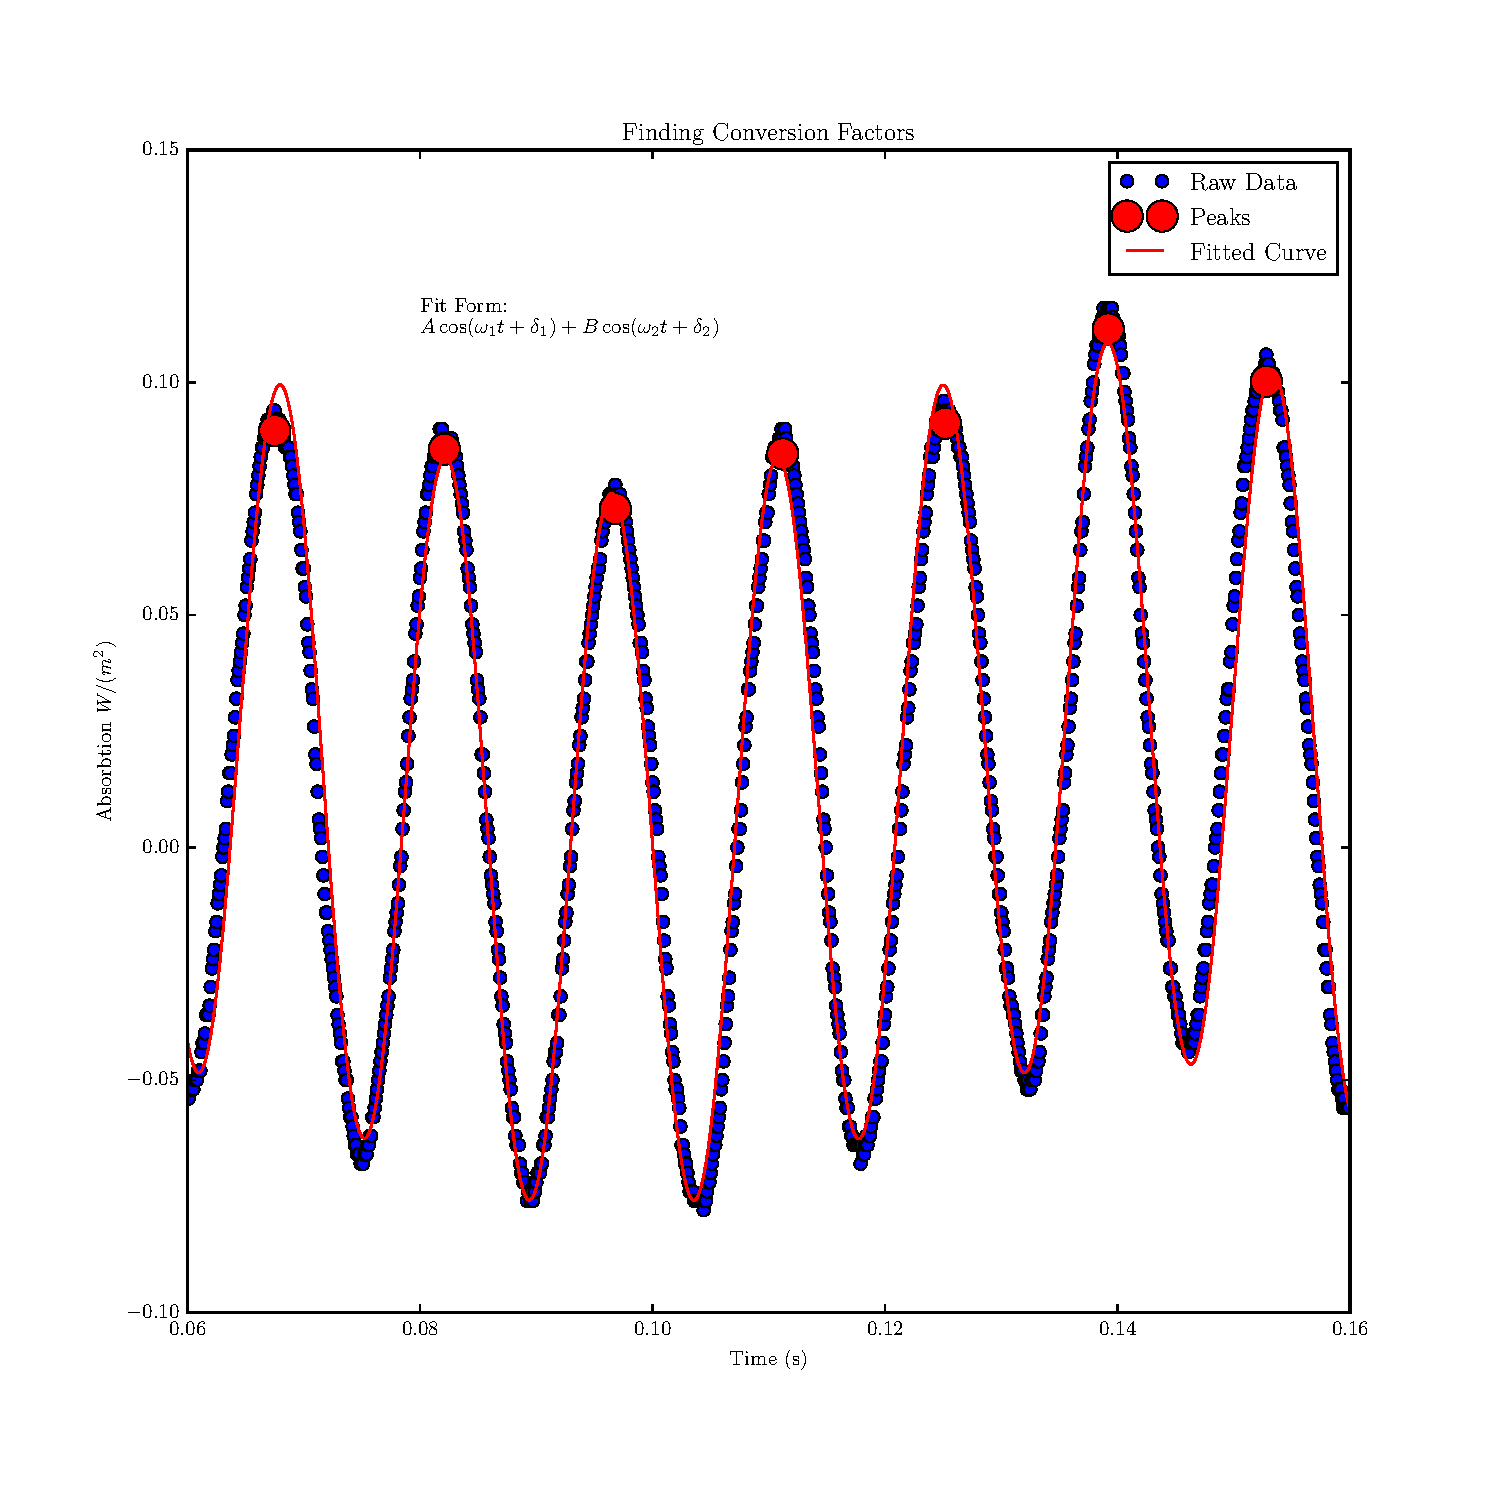
\includegraphics[scale=.75]{../plots/conversion.pdf}
    \caption{We have fit to the form shown in order to clean up the data.  From there, we have applied a gaussian filter for increasing values of the kernel standard deviation (see the documentation for numpy.gaussian\_filter for more information) in order to determine the correct coordinates for the peaks on the time axis.  The other axis is more or less irrelevant.  We have superimposed two cosine waves, because there appears to be some lower frequency oscillation in the system.  Since the fit is not crucial (we only use it as a first smoothing of the data to find the peaks), we do not cite a \redchi value, but visually the fit is good.  Also note that this is the cleanest part of the interferometer spectrum, and is shown because it is so clean.}
    \label{cal_graph}
  \end{figure}

  In order to get the other part of the conversion, we take the interference spectrum (Figure~\ref{cal_graph}), find the peaks and take the distances between them.  From our procedure used to find the peaks we can define the uncertainty in the peak locations as something like the standard deviation of the mean of the gaussian filter.  A very small number to be sure, but it is nonzero.  From this uncertainty and mean, we generate a random distribution of peak locations centered at each peak on the spectrum with a standard deviation of the error on each peak.  We then calculate differences between the peaks for each run (selecting a random point from this distribution each time) and average to find our best value.  The uncertainty in this value will simply be the standard deviation of the sample.  In order to properly populate the histogram we run this test 5000 times.

  \hspace{.25cm}

  Since the laser sweeps frequency (roughly) linearly, the conversion should be linear.  Thus, we have
  \begin{equation*}
    (\Delta f \pm \delta f) = k \times (\Delta t \pm \delta t).
  \end{equation*}
  Given the fact that we have values for $\delta t$ and $\delta f$, we calculate $k$ as:
  \begin{equation}
    k \pm \delta k = 55.5315 \, G\!H\!z/s \, \pm 5.73\%.
    \label{k}
  \end{equation}

  We can calculate the uncertainty in $k$ as the quadratic sum of the fractional uncertainty in t and f.  We use a quadratic sum because the uncertainty in f comes from an uncertainty in the length of the interferometer arms (again, propagated as a fractional uncertainty), while uncertainty in t comes from an uncertainty in the fit.

  \hspace{.25cm}

  The inquisitive reader might question why there isn't a constant offset in our determination for k.  Since we are only concerned with differences in time and frequency, such a constant offset would simply cancel anyway.  We must be careful - this calibration can only be used to relate \textbf{differences} in time to \textbf{differences} in frequency.  It is not an absolute conversion, nor is it perfect - the laser has idiosyncrasies that cause mode hops - a phenomenon that causes discontinuities in the spectrum and makes the saw tooth shape of the laser's frequency sweep distort significantly from the linear (modulo one period).  It is however, good enough especially when we can see that the region of interest is free of discontinuities.  So, we can use this value for $k$ in the future to make the necessary conversions.

\section{Data and Uncertainty Analysis}
  \subsection{Doppler Broadened Spectrum}
  The doppler-broadened spectrum is not very pretty, unfortunately~\ref{full_spectrum}.  We are simply using a version of the spectrum where the vapor cell is inside the interferometer to make alignment easier, as well as to clean up the spectrum.  The overall width of the peak (the large peak, not the hyperfine dips) is still the same as the doppler-broadened peak that would occur outside the interferometer, just easier to see.

  \begin{figure}[!htb]
    \centering
    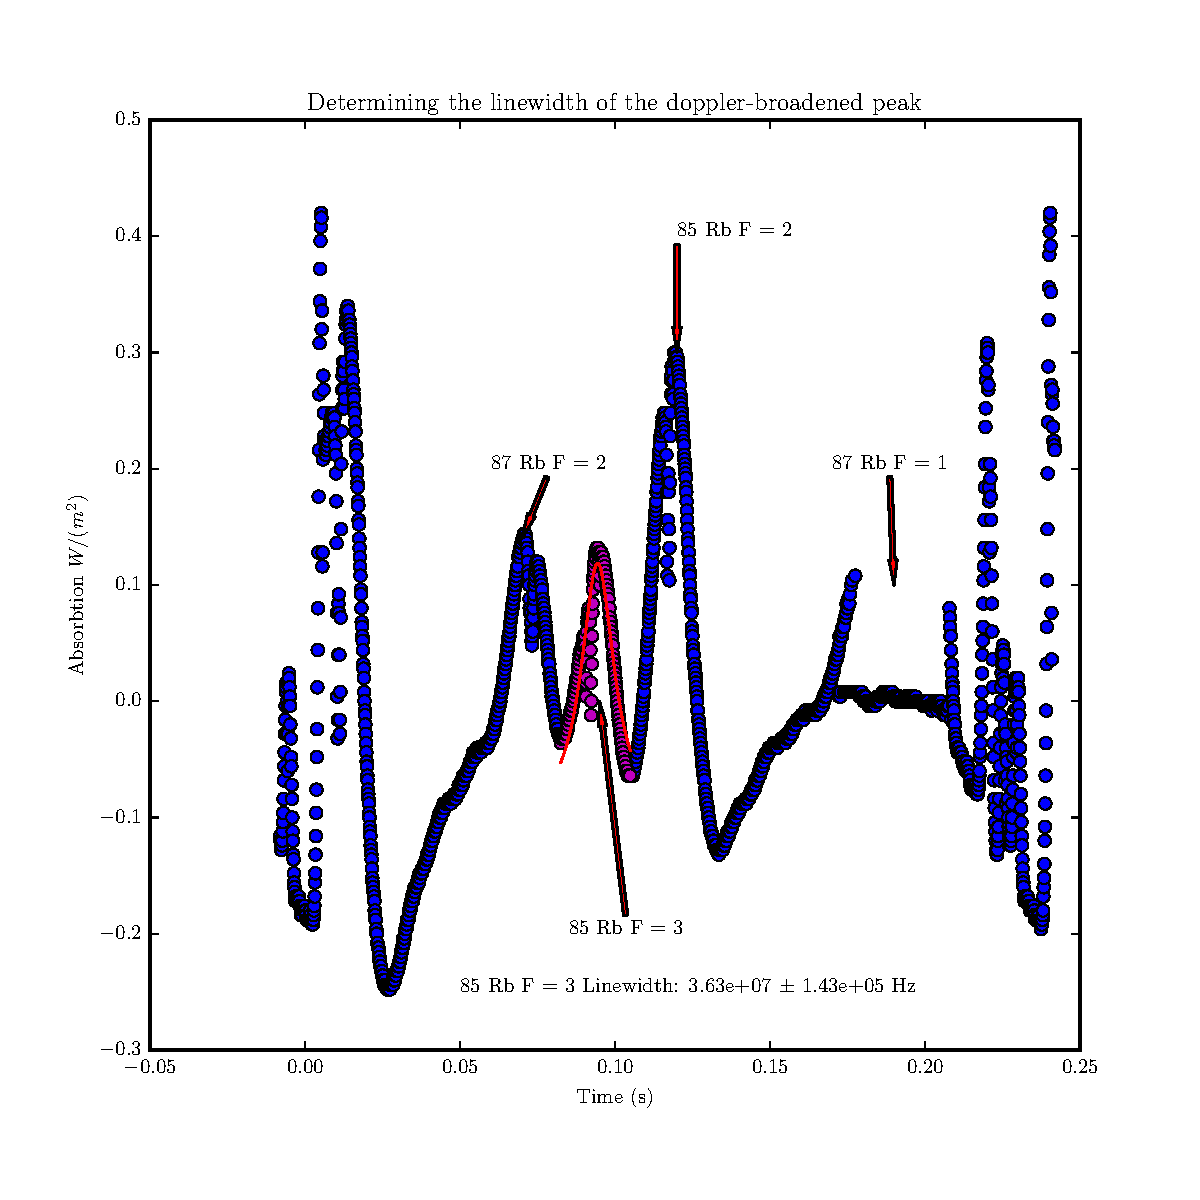
\includegraphics[scale=.75]{../plots/rb85_fwhm.pdf}
    \caption{For this fit we simply found the maximum again using a very rough gaussian filter and fit using manual adjustment of the other fit parameters.  The uncertainty in the linewidth comes from the covariance matrix element corresponding to the full width at half max of the fit form, suitably converted into frequency with Eq.~\ref{k} (taking into account uncertainty in k).}
    \label{full_spectrum}
  \end{figure}

  \hspace{.25cm}

  The 87Rb F = 1 peak has somehow collapsed - this is due to the fact that it is almost crashing into the laser's back sweep (the noise on either side).  Since this gave us the best resolution on the first three peaks, we decided to use this spectrum for further analysis.

  \hspace{.25cm}

  We can compare the measured doppler-broadened linewidth to a predicted value given by Eq.~\ref{doppler}.  Plugging in values, using 300K for room temperature and using the mass of a rubidium atom, we return the value $3.55 \times 10^7$ Hz, which corresponds nicely (but not exactly) to the measured value.  This is likely due to some other broadening mechanism, one possibility is that the temperature was slightly higher than what we expected, combined with the fact that we averaged masses of 85Rb and 87Rb could cause a broadening of this kind.  Another possibility is that the lasers were not perfectly aligned, that could also cause broadening of this sort.

  \subsection{Hyperfine Transitions}
  If we want to look closer at a given peak, we choose the 87Rb F = 2 peak.  We can zoom in and identify all the transitions, shown in Figure~\ref{hyperfine}.

  \hspace{.25cm}

  \begin{figure}[!htb]
    \centering
    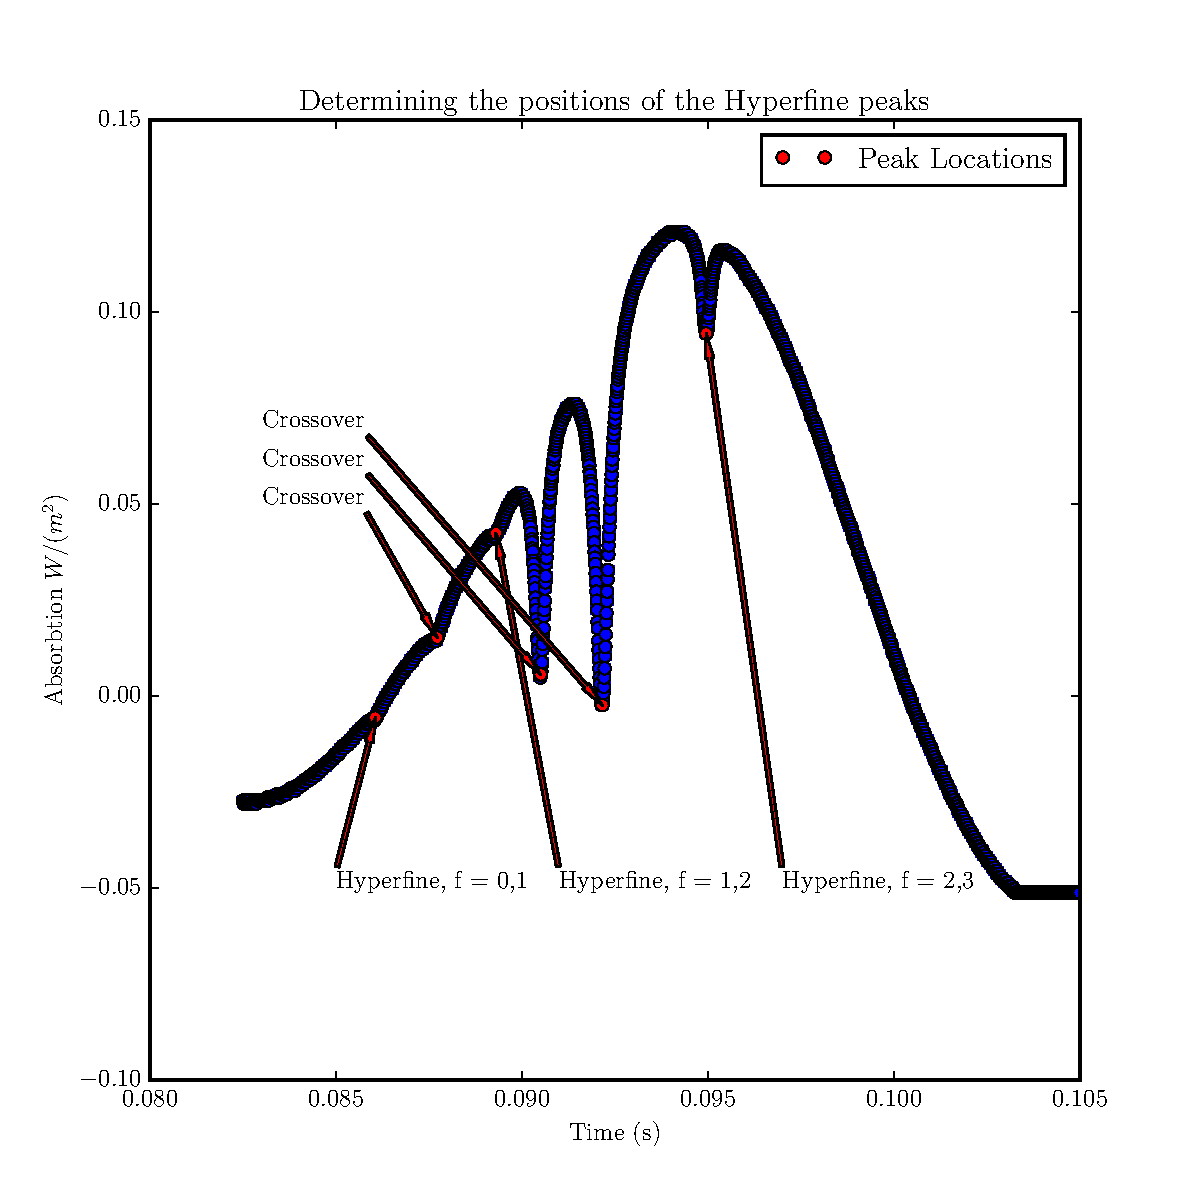
\includegraphics[scale=.75]{../plots/hyperfine.pdf}
    \caption{Finding the peaks exactly on this plot caused much consternation.  We found that in order to find the smaller peaks on the left, we had to first apply 5 iterations of the gaussian filter, and give each section a linear offset before being able to determine the local minimum that defined the peak.  The better-resolved peaks were quite simple, it was easy to apply a single filter and find the minimum that way.  Unfortunately, two of the very well-resolved peaks were crossover features, but sometimes that's just how life goes.}
    \label{hyperfine}
  \end{figure}

  There is some difficulty in determining uncertainty values for the peaks on this spectrum - since some of them are quite small and only barely visible, it is not entirely certain which part of the peak we are looking at.  Common sense tells us that we are likely looking at the very tip, but in practice this is not always true - we might be looking off to one side of the tip or something similar that might cause problems when trying to isolate the peak (the minimum of that neighborhood, suitably rotated).  If we are searching for the tip of the peak and can see the side of the peak, we might be seeing the transition from the hyperfine dip into the doppler-broadened peak instead of the tip of the peak.  Thus for the smaller peaks our uncertainty in the peak location is much larger than for the better-resolved peak.  What it essentially means is that for the smaller peaks, the uncertainty is dominated by peak location, while for the better-resolved peaks uncertainty is dominated by uncertainty in our conversion factor, $k$.

  \hspace{.25cm}

  In order to choose the hyperfine and crossover peaks, we make use of the fact that the crossovers occur exactly in between the hyperfine features.  Since the gap between the top two hyperfine features is large, there must be two crossover peaks in between them (one for the first and last hyperfine peaks, and one for the second and last).  The last one is trivial, the outermost peaks must be hyperfine and so the ones next to them must be crossovers.  Thus we can pinpoint exactly which peaks are which quite easily.

  \hspace{.25cm}

  In both cases we add uncertainties in quadrature, as again, the uncertainties are unrelated.  Both sources come from the fits, but because the two were calculated separately we can add the fractional uncertainties in quadrature and then apply that to the final value to extract uncertainty in said final value.  However, actually calculating differences in time (simple subtraction of the peak centers) between the peaks and adding the differences so that we find the difference between two hyperfine peaks and converting to frequency, we reach the following final values for the differences between the hyperfine transitions:

  \hspace{.25cm}

  \begin{table}[!htb]
  	\centering
  	\pgfplotstabletypeset[
     		every head row/.style={before row=\toprule, after row=\midrule},
     		every last row/.style={after row=\bottomrule},
     		columns/0/.style ={precision=0, column type = {|c|},column name=Frequency Differences (MHz)},
     		columns/1/.style ={precision=0, column type = {|c|}, column name=Uncertainties (MHz)},
        columns/2/.style ={precision=1, column type = {|c|}, column name=Literature Values (MHz)},
        columns/3/.style ={precision=1, column type = {|c|}, column name=Standard Deviations Away ($\sigma$)},
     		every even row/.style={before row={\rowcolor[gray]{0.9}}}]{../hyperfine_splitting.txt}
    \caption{Uncertainties are absolute.  The transitions are, in descending order, 0$\rightarrow$1, 1$\rightarrow$2, and 2$\rightarrow$3.}
    \label{hyperfine_splitting}
  \end{table}

  In reference to Figure~\ref{hyperfine}, obviously these values are not something that can simply be seen directly from the plot.  However, they do help to confirm which features are crossover and which are hyperfine transitions.  The fact that the values for the higher two states agree so well (within $1\sigma$!) indicates that our choices were well-motivated.  The first hyperfine feature, however, is off by almost $2\sigma$.  This would indicate some sort of error in either measuring the peak tip, or something else entirely.  To be perfectly candid, we are unsure as to what would have caused this error, but our most likely source is that the peak itself occurs at the very edge of the doppler peak.  This means that what we have found to be the peak tip may not, in fact, be the peak tip - the feature is not well resolved.  Due to time constraints we were unable to take more spectra, and so we are unfrotunately stuck.  However, it is very possible to take more spectra and find much more accurate values  from peaks that are better-resolved as we can see from the other two transition frequencies.

  \subsection{Single Hyperfine State Lifetime}
  Zooming in even further, we can focus in on one of the hyperfine dips.  We choose the one that is best-resolved, as we are zooming in quite close in order to avoid fitting the noise outside the peak.

  \hspace{.25cm}

  \begin{figure}[!htb]
    \centering
    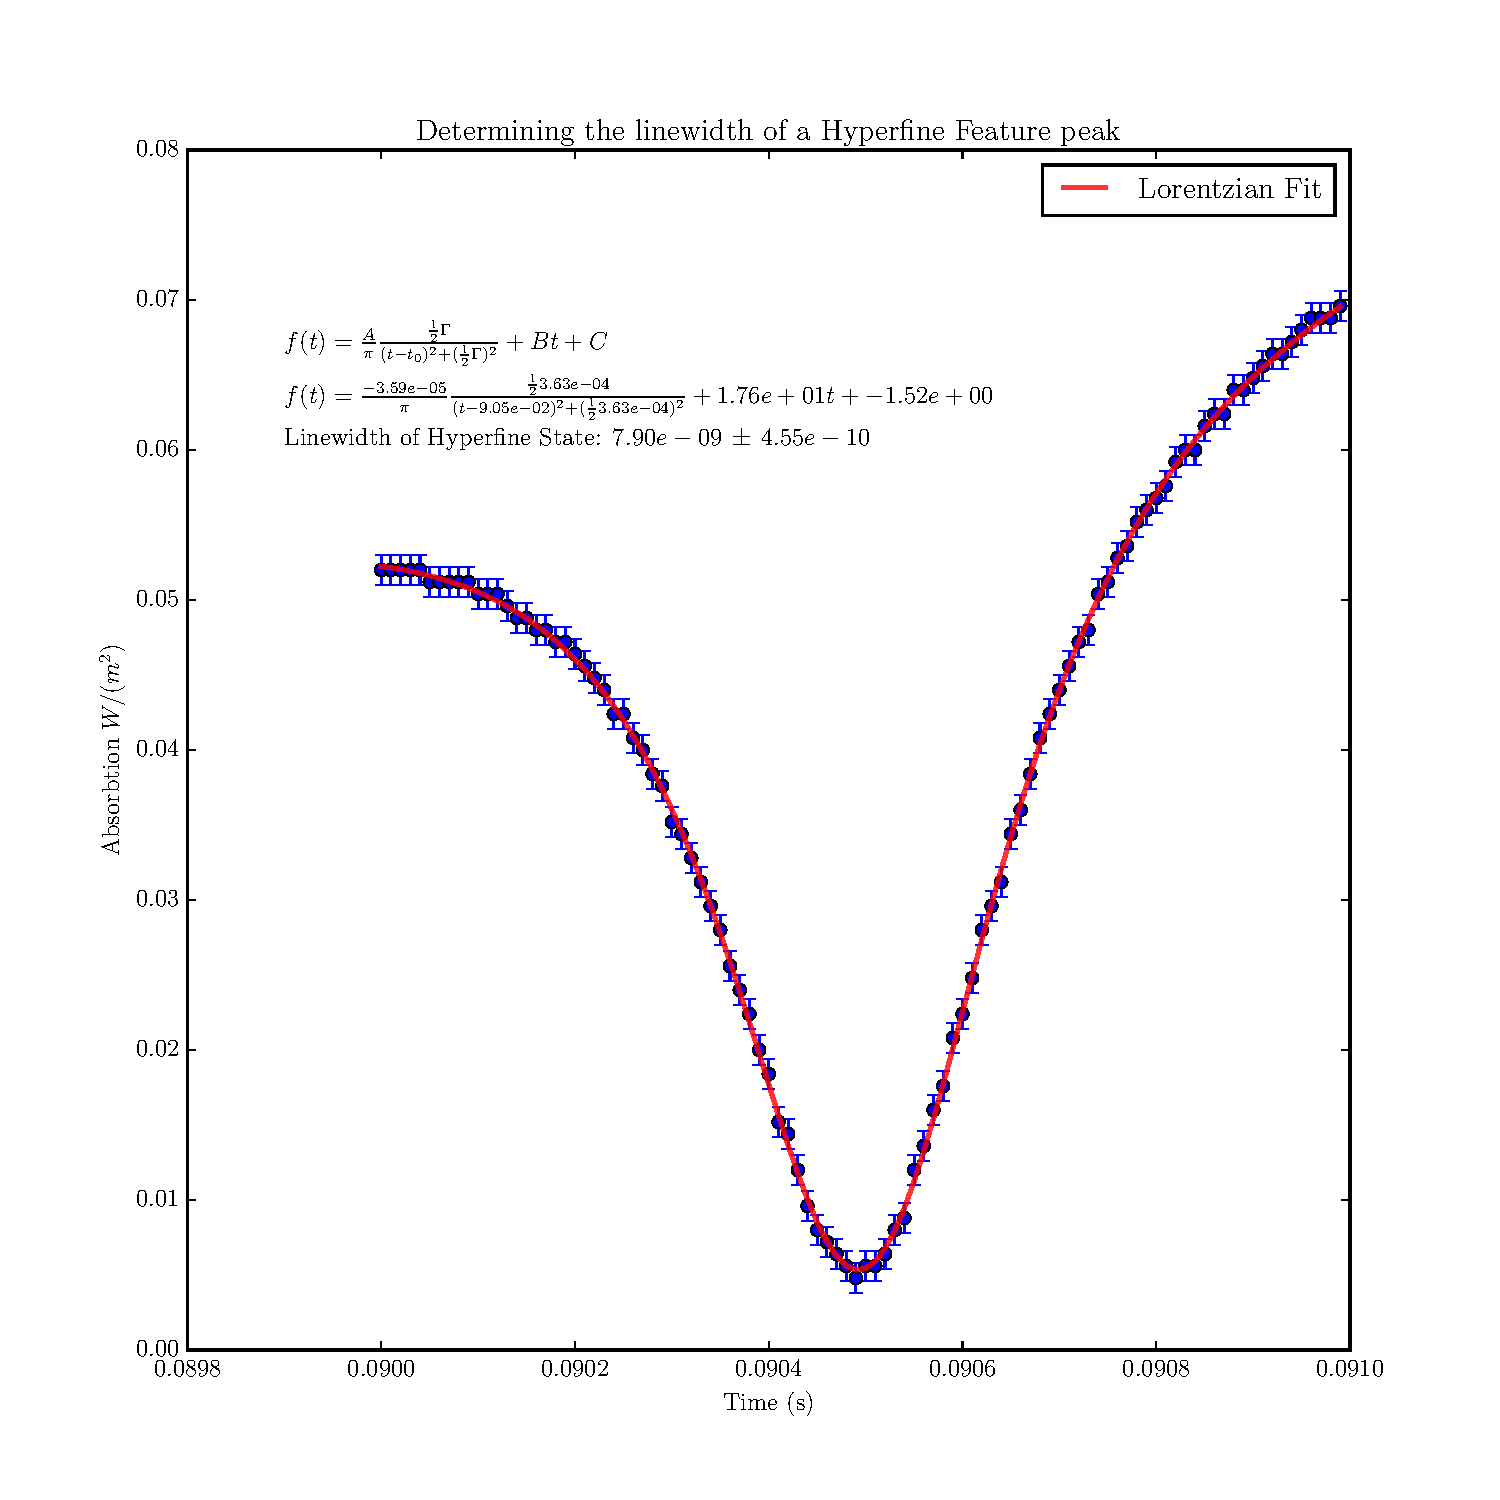
\includegraphics[scale=.75]{../plots/rb87_hyperfine.pdf}
    \caption{A simple fit form was employed here, we simply fit a Lorentzian form to the hyperfine feature.  We do not calculate the \redchi value because the covariance matrix diagonal elements were 2-3 orders of magnitude lower than the corresponding fit value, which would imply a very low \redchi value anyway.  Furthermore the off-diagonal elements were very nearly zero (of order $10^-7$) universally, which again indicates an excellent fit where the minimum of the parameter space is quite well defined.  The quoted uncertainty on the lifetime is dominated by the uncertainty in the conversion factor.}
    \label{lifetime}
  \end{figure}

  It is important to take a moment and ponder why the lifetime we measured is off from the lifetime that is generally accepted of 28 ns ($28\cdot10^{-9}$ sec).  We know that it's not due to any calculated uncertainty (as we can see), rather there is a physical effect that is causing   There are any number of broadening effects, in this case we have to narrow down which one caused this error.  In this kind of experiment, it is important to consider the fact that external fields can have a large impact on atoms in any state, and when they are already optically pumped, instead of shifting the states we will simply see broadening (especially in the uppermost energy level).  In this case, the experimental setup was such that the CCD camera was quite near to the vapor cell.  The stray electric fields within the vapor cell can and do cause Stark broadening, not enough to see the states split but enough to see the states broaden by quite a bit.  Since our value is not too far off - we are within an order of magnitude, we firmly believe that this is the reason for our lifetime decrease.

\section{Conclusion}
  In taking data we noticed that there were a few recurring sources of error that likely caused most of the broadening effects that we saw.  We hypothesize that the cause is Stark broadening due to stray fields coming from the CCD camera.  In aligning the laser, we had to find a good angle to ensure that the two laser points were well-aligned on the detector and their luminescences were well aligned in the vapor cell.  This necessecitated that we put the CCD quite close to the vapor cell, which is a strong source of broadening.  Another problem that likely caused broadening is that the vapor cell likely was not heated, which can cause accumulation of the rubidium atoms on the walls and lenses of the vapor cell, again causing broadening and other reflections.

  \hspace{.25cm}

  This work was undertaken in collaboration with Vasish Baungally.  Many thanks to the staff of the Advanced Undergraduate Physics Laboratory espeicially Aaron Mowitz for answering emails at times after midnight answering inane questions.

  \begin{thebibliography}{10}
    \bibitem{lab manual}
    	University of Chicago Department of Physics. "Hyperfine Spectroscopy of Rubidium"\\
    	https://wiki.uchicago.edu/display/P211manuals/Hyperfine+Spectroscopy+of+Rubidium. (Accessed Feb. 3-10, 2016)

    \bibitem{taylor}
    	Taylor, John. \emph{An Introduction to Error Analysis}. Sausalito: University Science Books, 1997.
  \end{thebibliography}

\end{document}
